\documentclass[tikz, border=3.14mm]{standalone}
\usepackage{pgfplots}
\pgfplotsset{compat=1.18}

\begin{document}
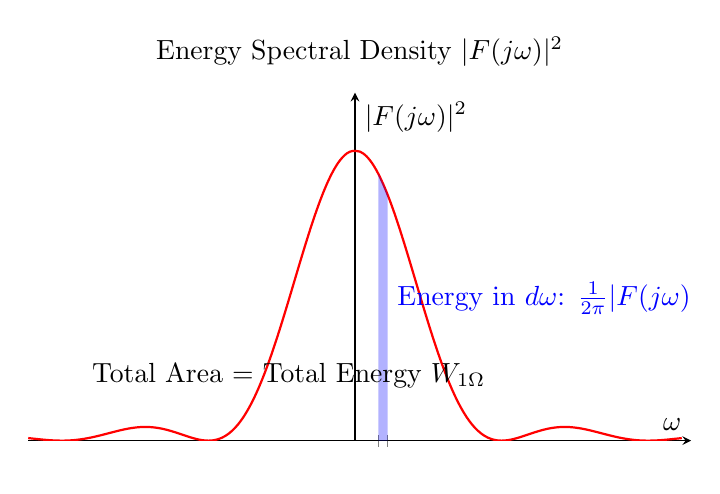
\begin{tikzpicture}
    \begin{axis}[
        axis lines = middle,
        xlabel = {$\omega$},
        ylabel = {$|F(j\omega)|^2$},
        xmin = -7, xmax = 7.2,
        ymin = 0, ymax = 1.2,
        xtick = {0.5, 0.7},
        xticklabels = {,},
        ytick = \empty,
        width = 10cm,
        height = 6cm,
        title = {Energy Spectral Density $|F(j\omega)|^2$}
    ]
        % Smooth curve: Sinc squared
        \addplot[thick, red, smooth, domain=-7:7, samples=200] {(sin(x*180/3.14)/(x))^2};
        
        % Shaded slice
        \addplot[fill=blue, fill opacity=0.3, draw=none, domain=0.5:0.7] {(sin(x*180/3.14)/(x))^2} \closedcycle;
        
        % Labels
        \node[anchor=south west, blue] at (axis cs:0.7, 0.4) {Energy in $d\omega$: $\frac{1}{2\pi} |F(j\omega)|^2 d\omega$};
        \draw[<->, blue] (axis cs:0.5, -0.05) -- node[below, pos=0.5] {$d\omega$} (axis cs:0.7, -0.05);
        
        \node[anchor=north east] at (axis cs:3, 0.3) {Total Area = Total Energy $W_{1\Omega}$};

    \end{axis}
\end{tikzpicture}
\end{document}
